\chapter{Results}

\section{Performance}

Performance of the RLS algorithm in terms of prediction accuracy
has been assessed offline for reasons of expediency,
using the notebook \textit{AssessPerformanceOffline.ipynb}.
Figure \ref{convergence} shows the error on example $(x_t, y_t)$
as a function of the simulation step $t$. For readability purposes,
the curves have been smoothed using a moving average with a window
size of 24.

\begin{figure}[H]
    \begin{center}
        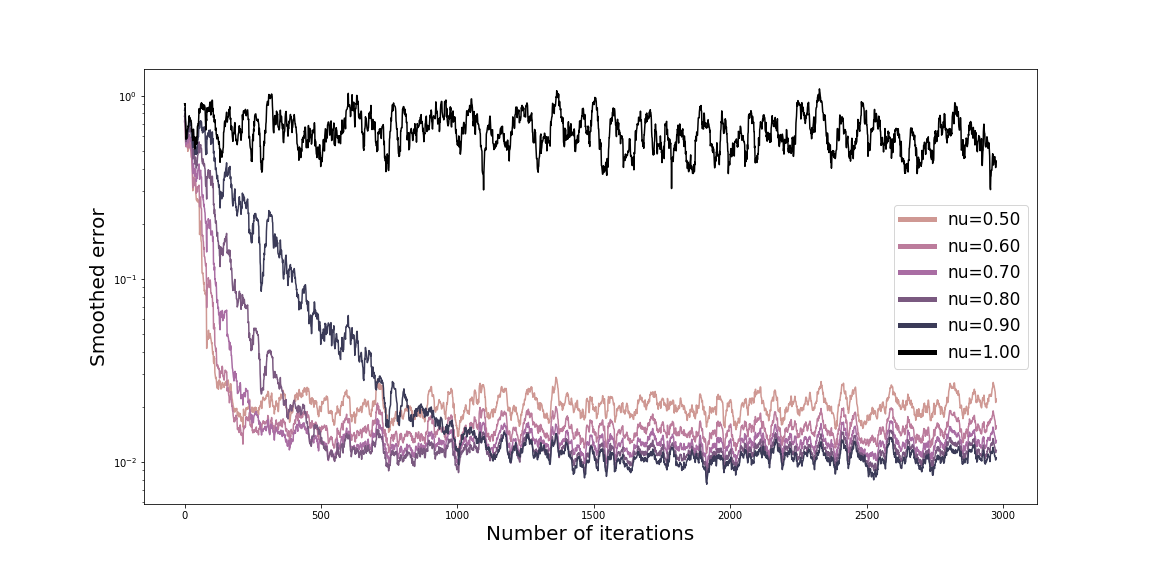
\includegraphics[width=\textwidth, keepaspectratio]{imgs/convergence.png}
        \caption{Convergence of RLS models with different forgetting factors, in log-scale.
            Darker curves are associated to models with higher forgetting factors.}
        \label{convergence}
    \end{center}
\end{figure}

As can be observed, models with higher forgetting factors exhibit slower convergence
but yield lower average errors in the long run. Also, a forgetting factor of $1$
seems to completely degrade the model's learning capabilities.

Since the simulations are made offline, the ground-truth coefficients are available
and can be used to better assess convergence. In figure \ref{frobenius},
the error has been replaced by the Frobenius norm of the difference between learnt
and ground-truth coefficient matrices. Differences in performance between the different
forgetting factors can be observed more clearly.

\begin{figure}[H]
    \begin{center}
        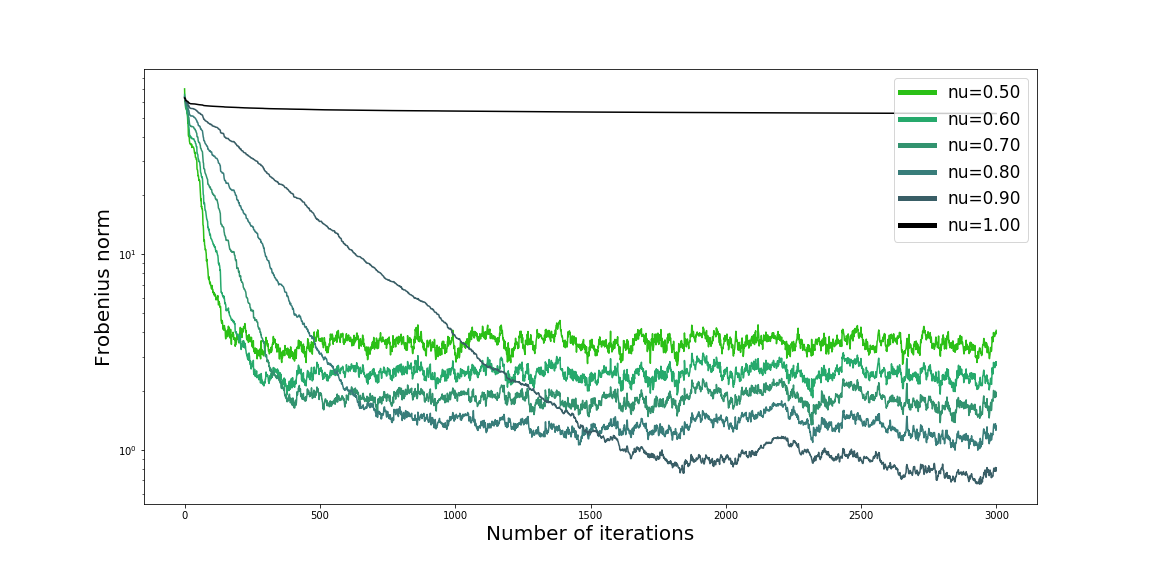
\includegraphics[width=\textwidth, keepaspectratio]{imgs/frobenius.png}
        \caption{Frobenius norm of the difference between learnt and ground-truth
            coefficient matrices across time, in log-scale. Darker curves are associated
            to models with higher forgetting factors.}
        \label{frobenius}
    \end{center}
\end{figure}


In figure \ref{stdv}, models were all run with a forgetting factor of 0.9 but
with different levels of Gaussian noise.
As can be reasonably expected, noisy models are harder to learn and yield
higher Frobenius norms. Surprisingly, it appears that
the relationship between Frobenius norm and noise levels is almost perfectly linear
(with some deviation).

\begin{figure}[H]
    \begin{center}
        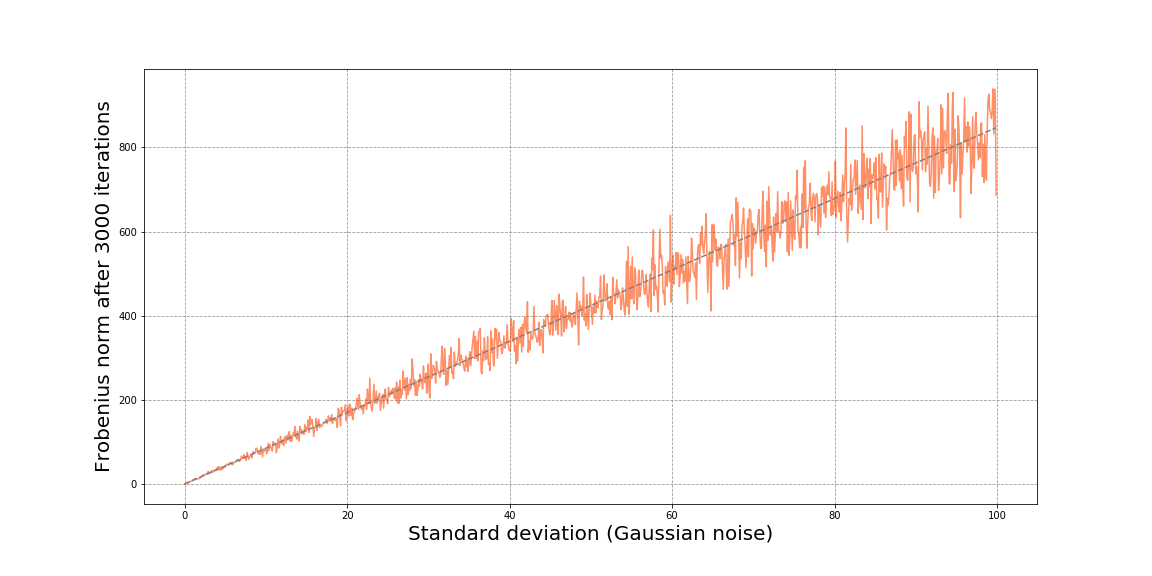
\includegraphics[width=\textwidth, keepaspectratio]{imgs/stdv.png}
        \caption{Frobenius norm after 3000 iterations, expressed as a function of
            the standard deviation of the Gaussian noise term.}
        \label{stdv}
    \end{center}
\end{figure}

Performance is not only affected by the noise level but also the number of
input variables, as shown in figure \ref{ninputs}. However, performance seems
to start increasing when the number of explanatory variables exceeds 20.

\begin{figure}[H]
    \begin{center}
        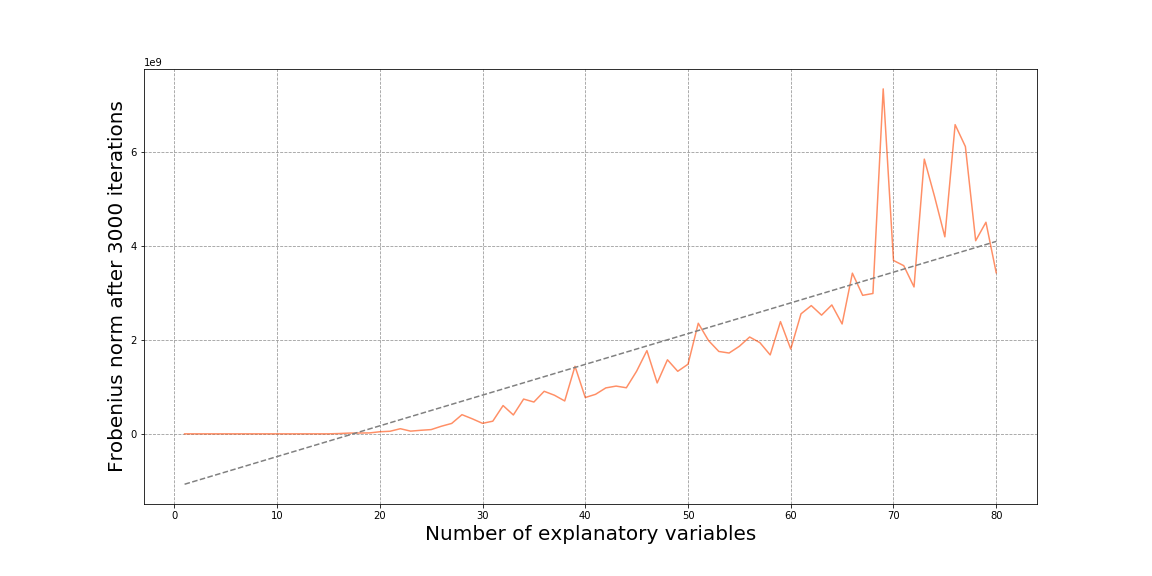
\includegraphics[width=\textwidth, keepaspectratio]{imgs/ninputs.png}
        \caption{Frobenius norm after 3000 iterations, expressed as a function of
            the number of explanatory variables in the model.}
        \label{ninputs}
    \end{center}
\end{figure}

It is a noteworthy that RLS exhibits extremely fast convergence~\cite{}.
As could be seen in figure \ref{convergence}, models with higher average errors
have the ability to convergence much faster than the others.
This phenomenon is better shown in figure \ref{convergencerate} below.

\begin{figure}[H]
    \begin{center}
        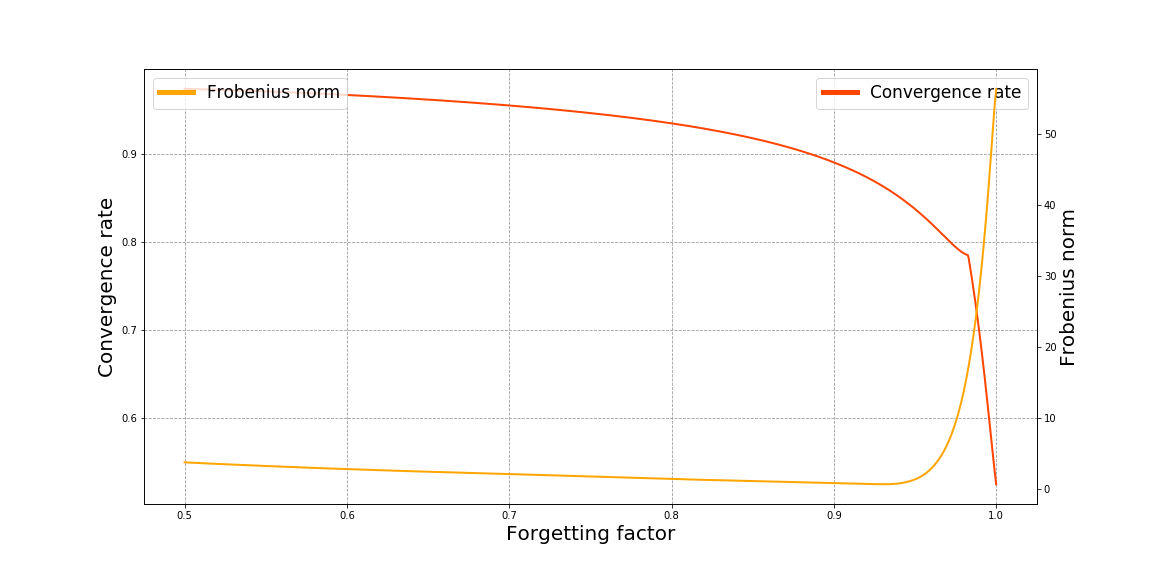
\includegraphics[width=\textwidth, keepaspectratio]{imgs/convergencerate.png}
        \caption{Convergence rates and Frobenius norms as functions of the forgetting factor.
            Both metrics are based on 3000 simulation steps. Convergence rate is related
            to the convergence of the prediction error.}
        \label{convergencerate}
    \end{center}
\end{figure}

Convergence rate has been computed as a function of the excess of error above the global minimum
across the whole learning process. The error is normalized and scaled in order to ensure that
the convergence metric is in the range $[0, 1]$.

\begin{equation}
    C_r(x) = 1 - \frac{1}{T} \int \frac{x - \min_i x_i}{\max_i x_i - \min_i x_i} dx
\end{equation}

Convergence rate decreases monotonically with the forgetting factor.
However, the frobenius norm after 3000 steps does not seem to be monotonic
but rather unimodal. In consequence, the value of the forgetting factor that
minimizes the Frobenius has been computed using a scalar optimization method.
Using the Brent method, a derivative-free technique efficient for finding global optima
in unimodal functions~\cite{basso1982iterative}, the minimum Frobenius norm is reached
when the forgetting factor is equal to 0.929.
